% Chapter 1

\chapter{Introducción general} % Main chapter title

\label{Chapter1} % For referencing the chapter elsewhere, use \ref{Chapter1} 
\label{IntroGeneral}

%----------------------------------------------------------------------------------------

% Define some commands to keep the formatting separated from the content 
\newcommand{\keyword}[1]{\textbf{#1}}
\newcommand{\tabhead}[1]{\textbf{#1}}
\newcommand{\code}[1]{\texttt{#1}}
\newcommand{\file}[1]{\texttt{\bfseries#1}}
\newcommand{\option}[1]{\texttt{\itshape#1}}
\newcommand{\grados}{$^{\circ}$}

%----------------------------------------------------------------------------------------

%\section{Introducción}
En este capítulo se exponen la motivación del cliente, sus objetivos y expectativas como así también una evaluación resumida del estado del arte.
%----------------------------------------------------------------------------------------
\section{Motivación}
\label{Motivación}

En la cultura norteamericana es habitual el plantear una residencia de retiro, el equivalente a la jubilación en países como la Argentina, en un lugar diferente a donde se ha desarrollado la vida profesional.
Es en este lugar donde muchas personas pueden dedicarse a realizar hobbies o actividades postergadas durante su vida profesional.

En este proyecto se desarrollará un vivero inteligente para el cultivo y crecimiento de plantines y su posterior trasplante a ser instalado en una casa de retiro en el estado de Carolina del Norte, Estados Unidos de América. 
En la figura 1 se observa un vivero hogareño típico de producción y dimensiones similares al propuesto.


La función principal del vivero será la de preparar diferentes especies de hortalizas para consumo, plantas ornamentales y/o decorativas junto con árboles para reforestación. Debido a esta diversidad de cultivos, la producción deberá ser sostenible a lo largo del año debiéndose poder adaptar las condiciones climáticas del vivero a las especies en cultivo. 

\begin{figure}[htpb]
\centering 
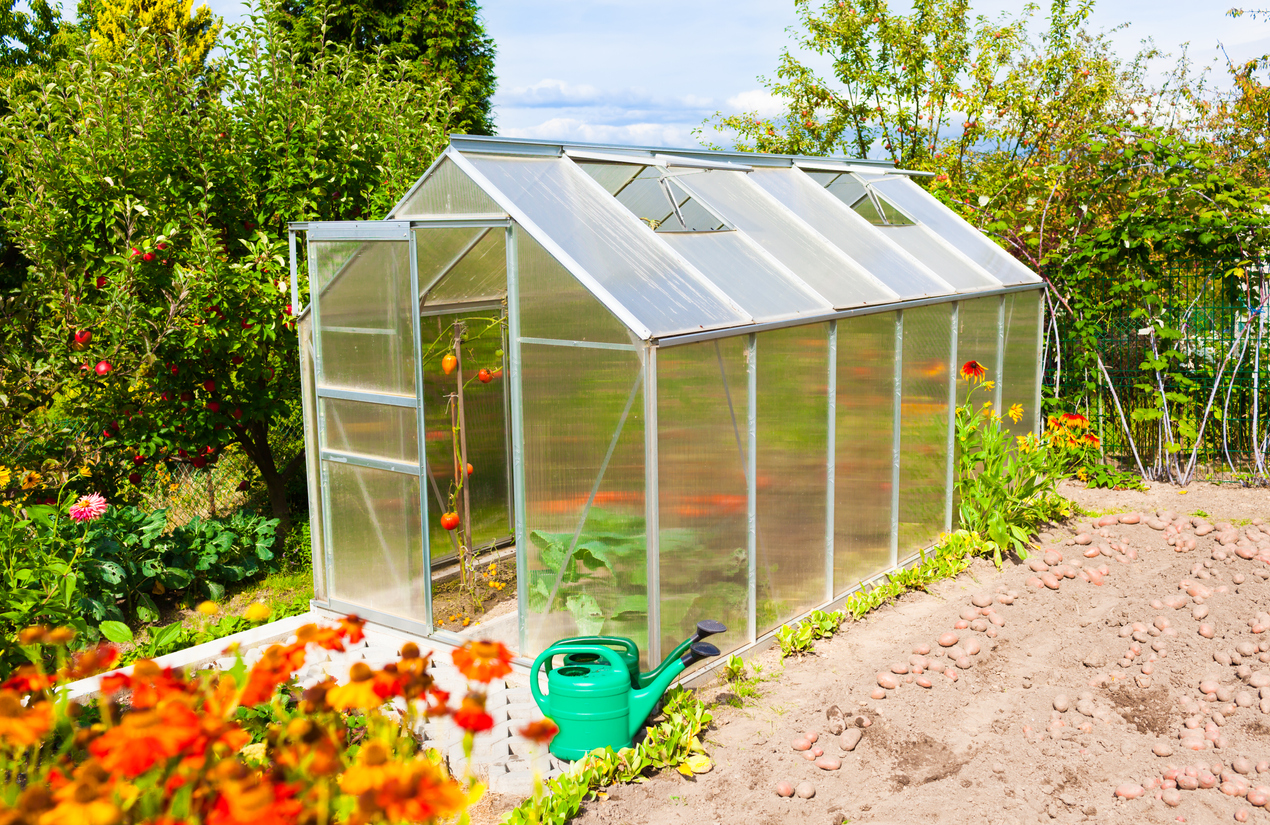
\includegraphics[width=.7\textwidth]{../Figures/invernadero1.jpg}
\caption{Invernadero hogareño}
\label{fig:imgInvernadero}
\end{figure}


%----------------------------------------------------------------------------------------

\section{Estado del arte}
\label{sec:Estado del arte}

Los viveros automatizados o inteligentes se han vuelto sumamente populares entre los aficionados y dueños de pequeños invernaderos debido a su capacidad de mejorar el crecimiento de las plantas minimizando la cantidad de trabajo manual requerido. Una de las características principales de un vivero inteligente es la capacidad de controlar automáticamente factores ambientales como la temperatura, la humedad, la luz y el riego. Esto se puede lograr mediante el uso de sensores, actuadores y controladores que pueden ajustar las condiciones en función de configuraciones preprogramadas o datos en tiempo real. 
En términos de control de temperatura, los viveros inteligentes pueden usar dispositivos como termostatos, ventiladores y calentadores para mantener el rango de temperatura ideal para el crecimiento de las plantas. La humedad se puede regular mediante humidificadores o deshumidificadores, mientras que la iluminación se puede controlar mediante el uso de temporizadores o sensores de luz. También se pueden implementar sistemas de riego controlados. En sistemas mas avanzados, se pueden controlar variables como el suministro de nutrientes, la regulación del dióxido de carbono y los sistemas de control de plagas. 




%\begin{table}[h]
%\centering
%\caption[Análisis del estado del arte]{Análisis del mercado.}
%
%\begin{tabular}{p{0.15\linewidth} | p{0.35\linewidth} | p{0.08\linewidth} | p{0.28\linewidth}}
%\toprule
%\textbf{Proveedor} & 
%\textbf{Características principales} & 
%\textbf{Costo} & 
%\textbf{Tamaño del mercado}\\
%\midrule
%Priva &
%  Sistemas integrales que incluyen gestión de clima, riego y energía.  &
%  \$\$\$\$ &
%  Grande, con una fuerte presencia en Europa y América del Norte. \\
%Hortimax &
%  Sistemas de control para clima, riego y gestión laboral.\ &
%  \$\$\$\$ &
%  Grande, con una fuerte presencia en Europa y Asia. \\
%Argus Controls &
%  Sistemas de automatización para clima, riego y fertirrigación.\ &
%  \$\$ &
%  Grande, con una fuerte presencia  América del Norte. \\ 
%Grodan &
%  Soluciones de riego, fertirrigación y control climático.\ &
%  \$\$ &
%  Grande, con una fuerte presencia en Europa y América del Norte. \\
%Heliospectra &
%  Sistemas de control de iluminación y aplicaciones agrícolas en interiores.\ &
%  \$\$\$\$ &
%  Pequeño, pero en crecimiento con presencia global. \\
%Growlink &
%  Controles inteligentes de temperatura, humedad, CO2, iluminación y riego.\ &
%  \$ &
%  Pequeño, pero en crecimiento con soluciones ajustables a cualquier tamaño. \\ 
%\bottomrule
%\hline
%\end{tabular}
%\label{tab:vendors}
%\end{table}


\begin{table}[h]
\centering
\caption[Análisis del estado del arte]{Análisis del mercado.}

\begin{tabular}{lcccccc} 
\toprule
%\textbf{Funcionalidad} & \textbf{Priva []} & \textbf{Hortimax []} & \textbf{Argus Controls []} &\textbf{Grodan []} & \textbf{Heliospectra []} & \textbf{Growlink []}\\
\textbf{Funcionalidad} & \textbf{Priva []}  & \textbf{Argus Controls []} &\textbf{Grodan []} & \textbf{Growlink []}\\

\midrule
Gestión de clima   & Sí & Sí & Sí & Sí \\
Control de riego   & Sí & Sí & Sí & Sí \\
Fertirrigación     & No & Sí & Sí & ? \\
Gestión de energía & Sí & ? & Sí & Si \\
Tamaño de mercado  & Grande &  Grande & Grande & Pequeño \\
Costo              & \$\$\$\$ &  \$\$ & \$\$ &  \$\$ \\
\bottomrule
\hline
\end{tabular}
\label{tab:vendors}
\end{table}

%----------------------------------------------------------------------------------------

\section{Objetivos y alcance}


El propósito de este trabajo es el desarrollo de un sistema de sensores y actuadores para el control de clima y riego de un vivero. Los mismos deberán comunicarse con una aplicación instalada en un servidor local donde se configurarán los parámetros y alarmas del sistema.

Con el propósito de disponer de un prototipo completo del sistema se incluyó:
 
\begin{itemize}
	\item Sistema para el monitoreo y control de dispositivos IoT.
	\item Sistema de control de usuarios, permisos y accesos a la plataforma.
	\item Interfaz gráfica para acceso y control de la plataforma.
	\item Instrucciones y/o tutoriales para facilitar el uso del sistema.
	\item Análisis, investigación y elección del hardware para los sensores y actuadores.


\end{itemize}


El presente trabajo no incluyó:
\begin{itemize}
	\item Implementación en sitio de los sistemas desarrollados.
	\item Implementación de métodos de control basados en condiciones climatológicas externas.
	\item Desarrollo o implementación de modelos analíticos o predictivos de las condiciones del vivero.
	\item Desarrollo o implementación de conexiones que no sean por Wi-Fi (LTE/5G). 
	
\end{itemize}